% Options for packages loaded elsewhere
\PassOptionsToPackage{unicode}{hyperref}
\PassOptionsToPackage{hyphens}{url}
\PassOptionsToPackage{dvipsnames,svgnames,x11names}{xcolor}
\documentclass[
  11pt,
]{article}
\usepackage{xcolor}
\usepackage[margin=0.9in]{geometry}
\usepackage{amsmath,amssymb}
\setcounter{secnumdepth}{-\maxdimen} % remove section numbering
\usepackage{iftex}
\ifPDFTeX
  \usepackage[T1]{fontenc}
  \usepackage[utf8]{inputenc}
  \usepackage{textcomp} % provide euro and other symbols
\else % if luatex or xetex
  \usepackage{unicode-math} % this also loads fontspec
  \defaultfontfeatures{Scale=MatchLowercase}
  \defaultfontfeatures[\rmfamily]{Ligatures=TeX,Scale=1}
\fi
\usepackage{lmodern}
\ifPDFTeX\else
  % xetex/luatex font selection
  \setmainfont[]{TeX Gyre Termes}
  \setmathfont[]{TeX Gyre Termes Math}
\fi
% Use upquote if available, for straight quotes in verbatim environments
\IfFileExists{upquote.sty}{\usepackage{upquote}}{}
\IfFileExists{microtype.sty}{% use microtype if available
  \usepackage[]{microtype}
  \UseMicrotypeSet[protrusion]{basicmath} % disable protrusion for tt fonts
}{}
\makeatletter
\@ifundefined{KOMAClassName}{% if non-KOMA class
  \IfFileExists{parskip.sty}{%
    \usepackage{parskip}
  }{% else
    \setlength{\parindent}{0pt}
    \setlength{\parskip}{6pt plus 2pt minus 1pt}}
}{% if KOMA class
  \KOMAoptions{parskip=half}}
\makeatother
\usepackage{longtable,booktabs,array}
\newcounter{none} % for unnumbered tables
\usepackage{calc} % for calculating minipage widths
% Correct order of tables after \paragraph or \subparagraph
\usepackage{etoolbox}
\makeatletter
\patchcmd\longtable{\par}{\if@noskipsec\mbox{}\fi\par}{}{}
\makeatother
% Allow footnotes in longtable head/foot
\IfFileExists{footnotehyper.sty}{\usepackage{footnotehyper}}{\usepackage{footnote}}
\makesavenoteenv{longtable}
\usepackage{graphicx}
\makeatletter
\newsavebox\pandoc@box
\newcommand*\pandocbounded[1]{% scales image to fit in text height/width
  \sbox\pandoc@box{#1}%
  \Gscale@div\@tempa{\textheight}{\dimexpr\ht\pandoc@box+\dp\pandoc@box\relax}%
  \Gscale@div\@tempb{\linewidth}{\wd\pandoc@box}%
  \ifdim\@tempb\p@<\@tempa\p@\let\@tempa\@tempb\fi% select the smaller of both
  \ifdim\@tempa\p@<\p@\scalebox{\@tempa}{\usebox\pandoc@box}%
  \else\usebox{\pandoc@box}%
  \fi%
}
% Set default figure placement to htbp
\def\fps@figure{htbp}
\makeatother
\setlength{\emergencystretch}{3em} % prevent overfull lines
\providecommand{\tightlist}{%
  \setlength{\itemsep}{0pt}\setlength{\parskip}{0pt}}
\usepackage[]{natbib}
\bibliographystyle{plainnat}
\usepackage{microtype}
\usepackage{fvextra}
\usepackage{xurl}
\usepackage{needspace}
\usepackage{fancyhdr}
\usepackage{caption}
\captionsetup{font=small,labelfont=bf}
\DefineVerbatimEnvironment{verbatim}{Verbatim}{breaklines=true,breakanywhere=true,fontsize=\footnotesize}
\setlength{\emergencystretch}{3em}
\setlength{\parskip}{0.35em}
\setlength{\parindent}{0pt}
\setlength{\headheight}{14pt}
\pagestyle{fancy}
\fancyhf{}
\fancyhead[L]{\small EvoTrace: Reflective Compression}
\fancyhead[R]{\small Research manuscript}
\fancyfoot[C]{\thepage}
\renewcommand{\headrulewidth}{0.3pt}
\usepackage{bookmark}
\IfFileExists{xurl.sty}{\usepackage{xurl}}{} % add URL line breaks if available
\urlstyle{same}
\hypersetup{
  pdftitle={EvoTrace: Evolving Tree-Structured Populations through Reflective Compression},
  pdfauthor={Anonymous authors},
  colorlinks=true,
  linkcolor={black},
  filecolor={Maroon},
  citecolor={black},
  urlcolor={blue},
  pdfcreator={LaTeX via pandoc}}

\title{EvoTrace: Evolving Tree-Structured Populations through Reflective
Compression}
\author{Anonymous authors}
\date{}

\begin{document}
\maketitle
\begin{abstract}
Evaluated programs have two distinct forms of value in automated
algorithm design: they provide starting points for further search, and
their development provides evidence for subsequent revisions. A program
can lose the first value while its history retains the second. We
introduce EvoTrace, which couples population updates with the reflective
compression of search experience. EvoTrace maintains a tree-structured
population of executable candidates, derivation relationships, and
condensed experience. A retention decision jointly determines the
programs that remain explicit, the regions of history to summarize, and
the retained locations that receive their experience. Contracted paths
and their removed side attempts contribute experience to reconnected
edges; other removed branches contribute experience to retained
ancestors. Later updates carry this experience forward as the tree
evolves. Refinement, crossover, and exploration read complementary views
of the same structure. EvoTrace makes the population an evolving
representation of both available programs and their design history, with
selection and reflection jointly determining how past evaluations remain
available to future search.
\end{abstract}

\subsection{1. Introduction}\label{introduction}

Large language models (LLMs) enable automated algorithm design (AAD)
through repeated program generation, evaluation, and revision
\citep{funsearch, eoh, elm}. Under a limited evaluation budget, each
trial produces two useful objects: an executable candidate and evidence
about a computational choice. The candidate supplies a starting point
for further search. The comparison with its parent can inform how a
later candidate should change. Search must continually decide which
implementations to develop and which experiences to bring into the next
design.

These decisions concern different forms of value. A program may be
superseded by a better descendant, while the revisions and alternatives
explored along its development remain informative. A regressed trial may
be a poor starting point, while its outcome helps interpret a later
modification of its parent. Candidate retention and experience retention
therefore need not select the same material. The central question is
\textbf{how a population can keep accumulating useful design experience
as its executable members change}.

Existing search states offer several ways to organize this material.
Evolutionary populations maintain candidates for variation
\citep{funsearch, eoh, partevo}. Reflective methods transform
evaluations into language feedback \citep{reevo}, and memory-based
methods organize experience across revisions or branches
\citep{deltaevolve, memorytree}. Tree and lineage methods preserve
derivation relationships for selection, generation, and pruning
\citep{mctsahd, pathwise, phyloevolve}. These approaches establish the
value of both candidate competition and developmental context. We focus
on the update connecting these decisions: using the retained candidate
structure to determine both the scope and the placement of experience
compression.

We view population update as a decision about how search history is
represented. Some implementations remain explicit because the search may
develop them further. Related history can instead continue as condensed
experience. \textbf{Reflection performs this compression, and a
tree-structured population gives it a scope and a location.} The tree
combines competition among executable candidates with the relationships
linking their development. Once the retained candidates are known, the
same structure identifies the intermediate histories between them and
the alternative branches around them. Those regions specify what to
summarize and where the result belongs.

We instantiate this idea in \textbf{EvoTrace}, an experience-bearing
tree-structured population maintained through \textbf{dynamic reflective
simplification}. Each update selects quality representatives and
recently developed implementations, then preserves the forks needed to
connect them. Removed intermediate versions and their side attempts
become experience on the reconnected edge. Other removed branches become
experience at a retained ancestor. Existing experience travels with its
carrier when a later update simplifies that carrier. Subsequent
generation draws both its starting program and its relevant history from
the maintained tree.

One retention decision specifies the surviving candidates, the regions
to compress, and their receivers. This supplies a structural link
between selection and experience accumulation: every removed region has
a definite recipient in the retained population. Parent sampling
allocates evaluations over the surviving candidates, and
operator-specific views provide local development for refinement, two
development paths for crossover, and route-level ideas for exploration.

Our contributions are twofold:

\begin{enumerate}
\def\labelenumi{\arabic{enumi}.}
\tightlist
\item
  \textbf{An experience-bearing tree-structured population.} We organize
  executable candidates, derivation relationships, and condensed design
  experience in one evolving structure, so that the population supplies
  both development starting points and their relevant history.
\item
  \textbf{Dynamic reflective simplification.} We couple population
  updates with experience compression. The retained structure jointly
  determines the history regions to summarize and their receiving nodes
  or edges, connecting removed attempts to subsequent generation.
\end{enumerate}

\subsection{2. Related Work}\label{related-work}

\textbf{Program evolution and candidate competition.} Genetic
programming evolves executable programs \citep{koza}, while
hyper-heuristics and algorithm configuration search over heuristic
components and solver settings \citep{hh, irace}. LLM-driven AAD extends
the variation process to program synthesis and revision
\citep{survey_aad}. Evolution through Large Models uses a code model for
mutation \citep{elm}, and language-model crossover recombines text-based
genotypes \citep{lmcrossover}. FunSearch combines program generation
with an island population \citep{funsearch}; EoH evolves heuristic
descriptions together with implementations \citep{eoh}. LLaMEA and
AlphaEvolve further develop evaluator-guided algorithm and code
evolution \citep{llamea, alphaevolve}. Candidate diversity and
allocation are addressed through harmony search \citep{hsevo}, niches
\citep{partevo}, and fitness-and-usage-based parent sampling
\citep{shinka}. EvoTrace adapts the latter sampler and couples candidate
maintenance to the compression of the associated design history.

\textbf{Derivation structure in algorithm search.} MCTS-AHD uses a
search tree and a tree-path reasoning action for heuristic generation
\citep{mctsahd}. Clade-AHD aggregates descendant evaluations into
beliefs for clade-level selection \citep{cladeahd}. PathWise combines an
outer population with an inner entailment graph and coordinated
planning, generation, and reflection \citep{pathwise}. PhyloEvolve
maintains a phylogenetic forest, an elite pool, trajectory-conditioned
generation, and structural pruning; its Summarizer periodically distills
trajectories into summaries retrieved by semantic similarity
\citep{phyloevolve}. These methods connect current candidates to their
derivations. EvoTrace uses the retained derivation structure to define a
joint update: path contraction and branch removal determine the regions
of reflection, and the resulting summaries remain on the retained
connections or ancestors that inherit those regions.

\textbf{Reflection and experience reuse.} Self-Refine iterates on
self-feedback \citep{selfrefine}; Reflexion and ExpeL retain language
experience across attempts \citep{reflexion, expel}. In AAD, ReEvo
combines short-term comparisons with long-term reflection \citep{reevo}.
RefineEvo uses planning and positive and negative experience
\citep{refineevo}, while MeEvo alternates population evolution with
reflection over shared history \citep{meevo}. DeltaEvolve organizes
changes as semantic deltas in a hierarchical context system
\citep{deltaevolve}. MEMOIR combines branch-local memory with summaries
distilled at branch termination \citep{memorytree}. EvoTrace connects
the scope and placement of reflection to the same retained structure
used for candidate maintenance. Its recursive handoff lets a summary
remain part of that structure as its original implementations leave the
online population.

\subsection{3. Method}\label{method}

\subsubsection{3.1. Problem and Overview}\label{problem-and-overview}

We consider AAD for a specified task interface. A candidate program
implements a designated function used by an enclosing solver. The
evaluator executes the program on a fixed search dataset and returns a
fitness value or failure feedback. We use the convention that lower
fitness is better. The search has a budget of \(B\) program evaluations,
including unsuccessful executions and repair evaluations. Model calls
for generation, repair, and reflection are accounted for separately.

EvoTrace maintains an explicit tree-structured population alongside a
complete attempt archive. The tree supplies selectable algorithms and
context for generation; the archive records generated programs,
evaluations, and population updates. Each iteration selects an
algorithm, generates and evaluates a candidate, attaches the final
evaluated version, and simplifies the updated population. The returned
program is the feasible archived program with the best search fitness,
with earlier creation order breaking ties. Any held-out evaluation is
performed after this choice.

\begin{figure}
\centering
\pandocbounded{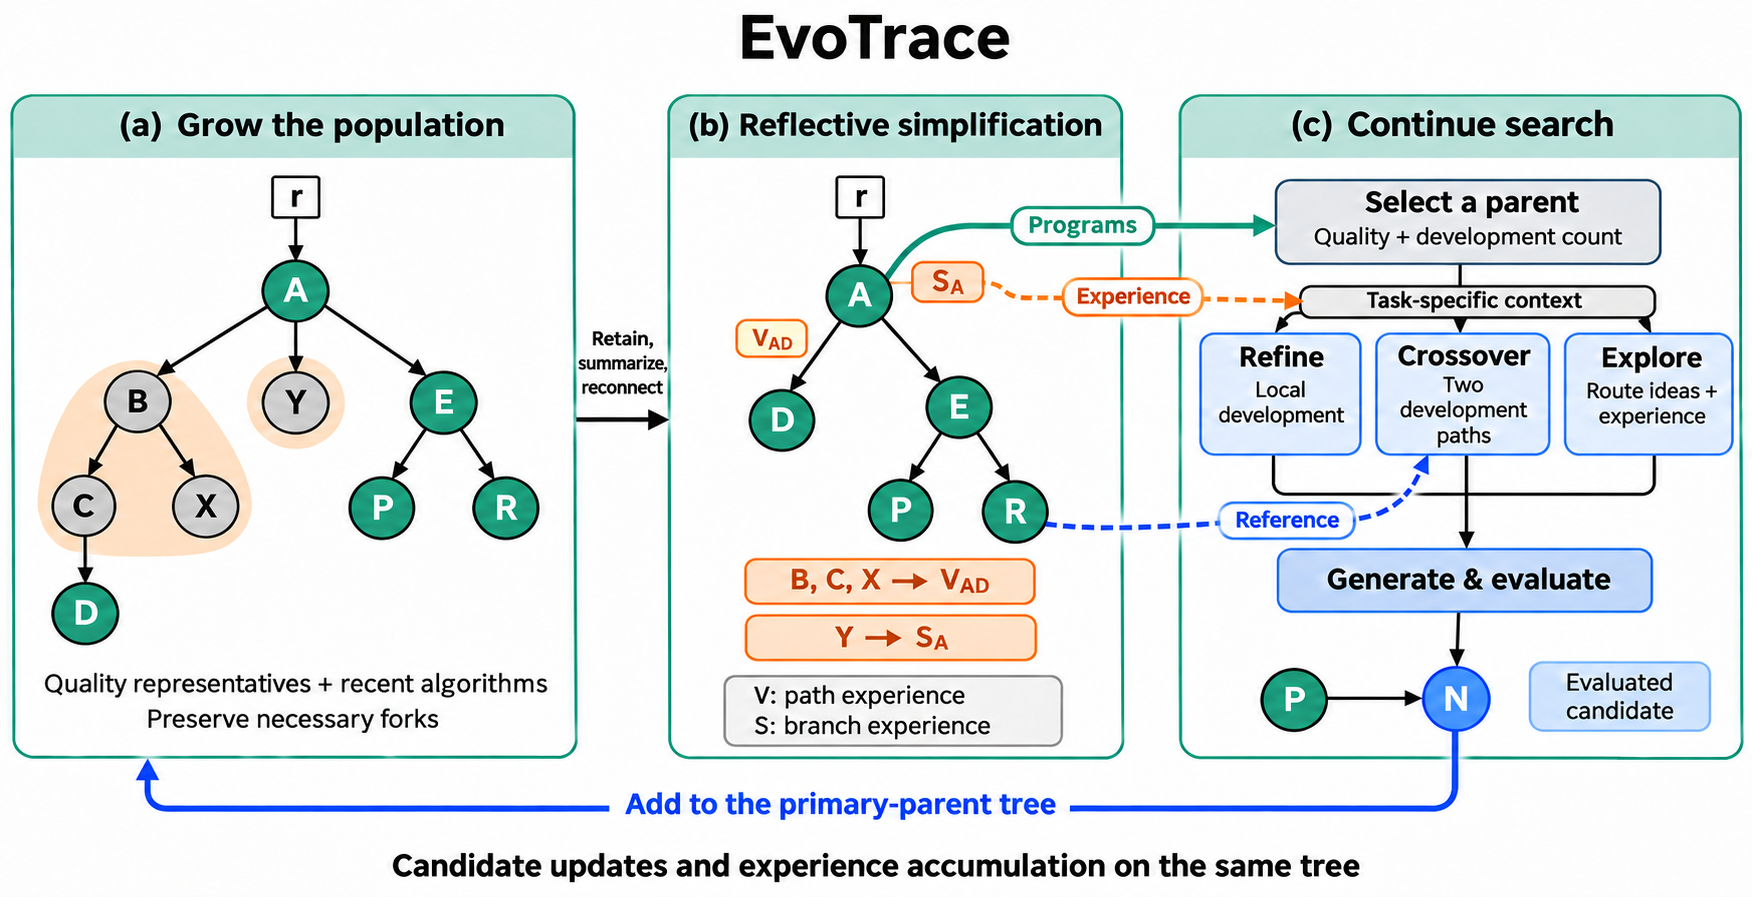
\includegraphics[keepaspectratio,alt={EvoTrace. A retained set determines how the population is simplified and where removed history becomes experience. The maintained tree supplies programs for selection and experience for task-specific context. Each attempt samples one operator; the evaluated candidate returns to the primary-parent tree. Dashed arrows show information inputs, including the crossover reference.}]{figures/framework.png}}
\caption{EvoTrace. A retained set determines how the population is
simplified and where removed history becomes experience. The maintained
tree supplies programs for selection and experience for task-specific
context. Each attempt samples one operator; the evaluated candidate
returns to the primary-parent tree. Dashed arrows show information
inputs, including the crossover reference.}
\end{figure}

\subsubsection{3.2. Tree-Structured
Population}\label{tree-structured-population}

Let \(T=(\mathcal N\cup\{r\},\mathcal E)\) be the current tree, where
\(r\) is a virtual root without an implementation. Each algorithm node
stores code, a description of its computation, fitness \(f(v)\) or
failure feedback, and usage records. Every node has one primary parent.
Crossover also records a reference algorithm as an auxiliary input; this
reference does not add a second edge to the maintained tree. All
retained feasible nodes, including internal nodes, can be selected for
further development.

The tree carries two forms of experience. \textbf{Selection experience}
\(S_v\), attached to a node, condenses side branches removed around that
location. \textbf{Variation experience} \(V_{uv}\), attached to an edge,
condenses the intermediate development and its removed side attempts
between retained endpoints. The names identify the simplification
operations that produce the summaries. Both types can describe
improvements, ties, regressions, and failures; a contracted path can
have a net regression. Selection experience informs generation and later
reflection, while parent sampling uses fitness and development counts.
The virtual root can carry selection experience from removed initial
routes. An ordinary edge represents one generation attempt. A contracted
edge represents a developmental stage and is marked accordingly.

Initialization and exploration start development routes; refinement and
crossover inherit the route of the primary parent. A route groups
implementations by their Init/Explore origin. Its identifier remains
with descendants when the original entry is removed. Routes organize
parent allocation and local context. An Explore entry may contract into
a descendant; a reconnected edge between different routes retains the
Explore label.

\subsubsection{3.3. Dynamic Reflective
Simplification}\label{dynamic-reflective-simplification}

Once initialization is complete, EvoTrace checks the population after
every evaluated addition. The update has three steps: select algorithms,
retain necessary forks, and partition the removed regions. All three
steps use the same tree snapshot before simplification.

\textbf{Selecting quality representatives.} Let
\(\mathcal P\subseteq\mathcal N\) contain the feasible nodes, ranked by
fitness and then creation order. Define rank quality as

\[
q(v)=1-\frac{\operatorname{rank}(v)}{\max(1,|\mathcal P|-1)},
\qquad v\in\mathcal P,
\tag{1}
\]

where the best node has rank zero. EvoTrace retains the best node and
considers the remaining candidates with \(q(v)\geq0.50\) in ranked
order. A candidate is superseded only by a strictly better descendant in
the same route; a superseded candidate does not join the representative
set, but can remain through recent use or fork retention. If removed,
its history enters the region determined by the final retained set. A
candidate is covered if an already selected representative has identical
normalized source or an abstract syntax tree (AST) distance below
\(0.08\). When the fitness values differ by at most \(10^{-9}\), the
distance threshold is \(0.20\). Otherwise, the candidate joins the
representative set \(\mathcal R\). Every representative used for
coverage has fitness no worse than the candidate being considered.

The distance is a multiset Jaccard distance over AST parent--child type
features and traversal bigrams. It retains operator types, called
function names, and control structure while omitting ordinary variable
identities and numerical values as feature values. Normalized-source
identity is a separate check that preserves variables and constants
while ignoring formatting, comments, and docstrings.

\textbf{Retaining recently used algorithms.} The evaluation clock \(t\)
counts actual program evaluations. Each feasible node has a last-use
time \(u(v)\), refreshed at birth or when an evaluated Refine or
Crossover attempt uses it as primary parent. Explore and read-only
reference use do not refresh this time. Let \(p(v)\) denote the parent
of \(v\) in the tree. The recent set is

\[
\mathcal U=\{v\in\mathcal P:t-\max(u(v),u(p(v)))<W\},
\qquad W=40,
\tag{2}
\]

where only \(u(v)\) is used when the parent is the virtual root or
belongs to a different route. Attempts from the same route may lose
recent eligibility together; quality representatives and necessary forks
remain retained.

Failed executions and repair evaluations advance the clock. Displaying a
node in context or retaining it as a structural connector does not
refresh its time. Recent retention preserves a candidate's eligibility
for continued development during the window; the parent sampler
determines its actual opportunities.

\textbf{Preserving necessary forks.} The retained set is

\[
\mathcal K=\{r\}\cup\mathcal R\cup\mathcal U
\cup\operatorname{LCA}(\mathcal R\cup\mathcal U),
\tag{3}
\]

Here, \(\operatorname{LCA}(A)\) denotes the set of lowest common
ancestors of pairs of nodes in \(A\), retaining the forks needed to
connect the selected nodes. Unary intermediate ancestors are eligible
for contraction. Quality representatives are determined before recent
retention and structural completion are added. Thus, a node retained
solely for recency or connectivity does not exclude a better candidate
from the representative set. The update computes ranks and
representatives once. The number of retained nodes follows recent use,
quality differences, and branching structure; the rule imposes no fixed
population cap.

\textbf{Partitioning paths and side branches.} For each retained
algorithm, EvoTrace finds its nearest retained ancestor in the original
tree. Removed intermediate nodes on this connection form a
path-contraction region. For each remaining removed node, the algorithm
walks upward to the first ancestor outside the remaining side-node set.
If that ancestor is a contracted intermediate, the side node joins its
path region; otherwise, its retained ancestor or the root receives a
side-branch region. Each removed node belongs to exactly one region in
that update. Multiple side branches assigned to the same receiver are
processed together.

This partition can shorten a path and remove its side branches in the
same update. Consider \(A\rightarrow B\rightarrow C\rightarrow D\), with
branches \(B\rightarrow X\) and \(A\rightarrow Y\), when only \(A\) and
\(D\) remain. Nodes \(B,C\) belong to the contracted path, and \(X\)
joins that same path region, contributing to \(V_{AD}\). Branch \(Y\)
updates \(S_A\) at \(A\). Earlier experience attached to \(B\) or \(C\)
travels with those nodes into the path region.

\begin{figure}
\centering
\pandocbounded{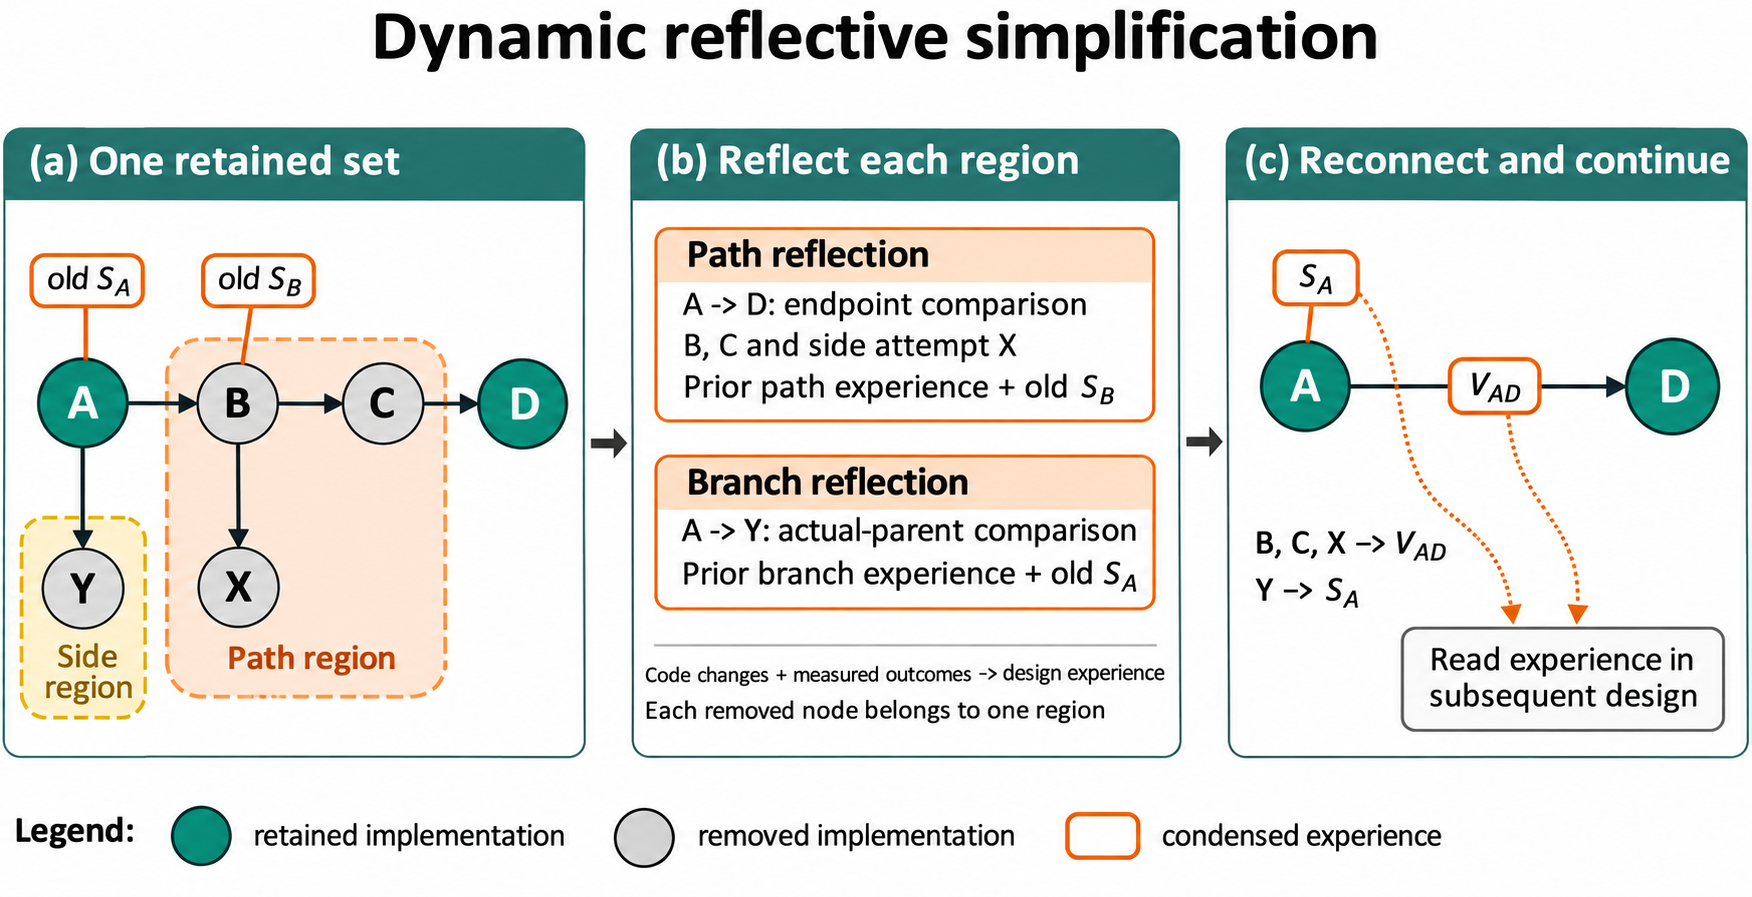
\includegraphics[keepaspectratio,alt={Experience follows the retained structure. With A and D retained, intermediate versions B and C and side attempt X form one path region, summarized on the reconnected edge as V\_\{AD\}. The separate branch Y updates S\_A. Earlier experience travels with its carrier: old S\_B enters the path summary, while old S\_A merges with Y.}]{figures/reflective-simplification.png}}
\caption{Experience follows the retained structure. With A and D
retained, intermediate versions B and C and side attempt X form one path
region, summarized on the reconnected edge as \(V_{AD}\). The separate
branch Y updates \(S_A\). Earlier experience travels with its carrier:
old \(S_B\) enters the path summary, while old \(S_A\) merges with Y.}
\end{figure}

\subsubsection{3.4. Region Reflection}\label{region-reflection}

\textbf{Region-specific reflection.} EvoTrace makes one reflection call
for each final contraction region and each grouped side-branch region. A
path reflection receives retained endpoint implementations, their net
difference, intermediate implementations and outcomes, their removed
side attempts, and inherited node and edge experience. A side-branch
reflection receives the receiver's implementation when available, the
removed attempts and their actual parent-relative differences,
evaluation or error feedback, and earlier relevant experience. The
virtual root supplies a task-level origin when there is no retained
algorithm receiver. Contracted inputs are explicitly presented as stages
of development. Side-branch comparisons use each trial's actual parent.
Current comparisons are supplied as program-computed outcome labels; raw
scores remain in the archive and the program attaches endpoint scores to
path experience. Both prompts distinguish an Explore draft from local
tuning and attribute each observed outcome to the evaluated
implementation.

The reflection prompt asks for a concise account of the tested
computations and their observed outcomes, followed by a tentative
explanation when supported. It distinguishes net start-to-end changes
from intermediate comparisons and treats jointly modified components as
a combined change. The prompt asks the model to keep earlier experience
where it remains consistent with the measured comparisons; the
comparison labels themselves are computed by the program. Generated
design rationales are excluded from the evidence. All regions in one
update read the same original snapshot; newly produced summaries are not
reused within that pass.

Path reflection updates \(V_{uv}\) on the reconnected edge. Side-branch
reflection updates \(S_u\) at the receiver, incorporating its existing
selection experience. When a later update removes a carrier, its
accumulated experience enters the appropriate new region. This recursion
retains a condensed account of development while allowing intermediate
implementations to leave the explicit population. The tree stores these
textual summaries alongside retained implementations; the attempt
archive preserves the complete underlying evidence.

\subsubsection{3.5. Search from the Maintained
Tree}\label{search-from-the-maintained-tree}

\textbf{Parent and reference selection.} EvoTrace adapts the weighted
parent sampler of ShinkaEvolve \citep{shinka}. Let \(D(v)\) denote the
route containing \(v\), identified by its original Init/Explore
identifier. Each nonempty route contains its retained feasible nodes.
Their weights and sampling probabilities are

\[
w(v)=\sigma\!\left(10\frac{m-f(v)}{s}\right)\frac{1}{1+c(v)},
\tag{4}
\]

\[
P(D)\propto\max_{u\in D}w(u),\qquad P(v\mid D)=\frac{w(v)}{\sum_{u\in D}w(u)},
\tag{5}
\]

where \(\sigma\) is the sigmoid function, \(c(v)\) counts evaluated
Refine and Crossover attempts using \(v\) as primary parent, and \(m\)
and \(s\) are the median and median-absolute-deviation scale of fitness
over quality representatives, recomputed on the current tree before each
sampling step. All retained feasible nodes remain eligible, with
probability \(P(D(v))P(v\mid D(v))\). At fixed weights, adding a version
whose weight does not exceed its route maximum leaves the route
probability unchanged. In an actual search update, probabilities can
change through a new maximum, further development of a parent, or a
shift in the representative set and its normalization.

After selecting a parent, EvoTrace samples Refine, Crossover, or Explore
with probabilities \(0.45\), \(0.25\), and \(0.30\), respectively.
Crossover first excludes the parent and normalized-source duplicates,
then applies the rank-quality rule to the available references.
Candidates with quality at least \(0.30\) are eligible. EvoTrace prefers
an unused ordered parent--reference pair and chooses the largest AST
distance within that pool, breaking ties by fitness and creation order.
It permits pair reuse once all eligible pairs have been used and uses
Refine when no eligible reference exists.

\textbf{Context at the scale of the design decision.} The three
operators read different views of the same population:

{\def\LTcaptype{none} % do not increment counter
\begin{longtable}[]{@{}
  >{\raggedright\arraybackslash}p{(\linewidth - 4\tabcolsep) * \real{0.3333}}
  >{\raggedright\arraybackslash}p{(\linewidth - 4\tabcolsep) * \real{0.3333}}
  >{\raggedright\arraybackslash}p{(\linewidth - 4\tabcolsep) * \real{0.3333}}@{}}
\toprule\noalign{}
\begin{minipage}[b]{\linewidth}\raggedright
Operator
\end{minipage} & \begin{minipage}[b]{\linewidth}\raggedright
Structural context
\end{minipage} & \begin{minipage}[b]{\linewidth}\raggedright
Current design task
\end{minipage} \\
\midrule\noalign{}
\endhead
\bottomrule\noalign{}
\endlastfoot
Refine & Current code and fitness; formation path within the current
route and a brief account of its source; node selection experience;
visible outgoing trials or developmental stages & Revise the current
computation using its development and evaluated alternatives \\
Crossover & Both implementations; their common ancestor and diverging
paths within a route, or separate local development paths across routes;
relevant node and edge experience; outgoing trials from the primary
parent & Decide which computations to transfer and how to integrate
them \\
Explore & Distinct route-entry ideas; the most recently generated
retained version in each selected route; node and edge experience; root
experience; one existing implementation & Construct an alternative with
a different main computation \\
\end{longtable}
}

An ordinary transition supplies a difference relative to its actual
parent and its outcome. A contracted transition supplies endpoint
outcomes and accumulated variation experience. Difference sequences
include the baseline code needed to interpret them. Within a route,
Crossover presents the common ancestor once. Across routes, it
summarizes shared provenance without expanding earlier routes. Explore
labels the source of each experience without repeating the full design
description. Exploration organizes ideas and experience before showing
an existing implementation, allowing the model to reconsider its
representation or procedure.

The context builder first assembles the relevant retained material. If a
generation prompt exceeds its input budget, it reduces complete entries
from path, trial, or route views according to the actual tokens
released. Current code, reference code, and required difference
baselines remain available. Context fitting changes a prompt view; it
does not change the tree, retention decisions, or experience ownership.
Each operator returns a complete implementation and a description of its
computation.

\subsubsection{3.6. Search Procedure}\label{search-procedure}

Algorithm 1 summarizes the search. Initialization creates five feasible
programs under the same evaluation budget. Each generation attempt has
at most one repair opportunity and contributes at most one final
evaluated node. Repair re-evaluation consumes budget separately.
Attempts that produce no program evaluation do not enter the tree or
advance its clock.

\par\noindent\begin{minipage}{\linewidth}
\begin{verbatim}
Algorithm 1: EvoTrace
Input: task interface, evaluator, LLM, evaluation budget B
Create a virtual root, an empty population, and an attempt archive
while evaluation budget remains and the stopping rule is not met:
    if fewer than five feasible initial programs have been obtained:
        build an initialization prompt
    else:
        sample a parent and operator; choose a reference when needed
        build and fit the corresponding tree-context view
    generate and evaluate a program, allowing at most one repair
    record all requests and evaluation outcomes
    if the attempt contains an evaluated program:
        attach its final evaluated version; update actual-use records
        if initialization is complete:
            select representatives and recent nodes on one snapshot
            add necessary branching ancestors to obtain the retained set
            partition removed paths and side branches on that snapshot
            reflect on each region
            reconnect retained nodes and attach the resulting experience
    commit the attempt and its population update
return the feasible archived program with the best search fitness
\end{verbatim}
\end{minipage}


The update preserves the best current algorithm and reconnects every
retained node to its nearest retained ancestor. Pairwise fork closure
ensures that contracted intermediate paths are disjoint; the remaining
removed nodes have a unique receiving region. Appendix B gives the
argument for these structural properties.

\subsection{4. Preliminary Evaluation}\label{preliminary-evaluation}

We examine the implementation on four combinatorial optimization tasks
and report a frozen early-search snapshot. The snapshot contains 12
independent runs, with seeds 0, 1, and 2 for each task, from the
source-frozen deployment of 14 November 2026. Each run has a target
budget of 1,000 evaluations. At the snapshot, runs have completed 62--97
evaluations. We report training fitness at the common 60-evaluation
checkpoint and analyze the population updates committed in each observed
prefix. Held-out performance and complete-search comparisons require the
completed runs.

\subsubsection{4.1. Tasks and Evaluation
Conditions}\label{tasks-and-evaluation-conditions}

Each task evolves a function within a fixed solver. TSP evolves
next-node selection in sequential tour construction. CVRP and OP evolve
edge priors for ant colony optimization. FSSP evolves the matrix and
job-selection computation used by guided local search. Objectives are
mean tour length, mean route length, mean makespan, and negative mean
collected reward, respectively. All four objectives are minimized.

Search uses 16 training instances per task. A disjoint set of 50
same-scale instances is reserved for testing the final selected program.
Each complete training evaluation has a shared 160-second time limit and
a 2 GiB process memory limit; the evaluator uses one worker. Failures
consume evaluation budget, and repair re-evaluations are counted
separately. The model pool serves Qwen3.8-27B with native thinking
disabled. Generation uses temperature 1.0 and at most 16,384 output
tokens; reflection uses temperature 0.3 and at most 1,536 output tokens.
Appendix D records the remaining task and sampling settings.

After search, the best feasible training program is fixed before
testing. Test results do not affect selection. Model requests and
reported token usage are accounted for separately from program
evaluations. This separates the cost of experience compression from the
evaluation budget used for search.

\subsubsection{4.2. Training Fitness at a Common
Budget}\label{training-fitness-at-a-common-budget}

Table 1 reports the best training fitness after 60 evaluations. Standard
deviations are sample standard deviations over the three independent
search seeds. Scores retain their native units; OP is negative because
the evaluator minimizes the negative collected reward.

\Needspace{12\baselineskip}
\begin{longtable}[]{@{}lrrr@{}}
\caption{Best training fitness at 60 evaluations. Lower is
better.}\tabularnewline
\toprule\noalign{}
Task & Seeds 0 / 1 / 2 & Mean & SD \\
\midrule\noalign{}
\endfirsthead
\toprule\noalign{}
Task & Seeds 0 / 1 / 2 & Mean & SD \\
\midrule\noalign{}
\endhead
\bottomrule\noalign{}
\endlastfoot
TSP & 5.8774 / 5.9590 / 5.9229 & 5.9198 & 0.0409 \\
CVRP & 8.5584 / 8.6008 / 8.7791 & 8.6461 & 0.1171 \\
FSSP & 3880.31 / 3879.12 / 3892.25 & 3883.90 & 7.26 \\
OP & -14.2787 / -14.5994 / -14.2663 & -14.3815 & 0.1888 \\
\end{longtable}

\begin{figure}
\centering
\pandocbounded{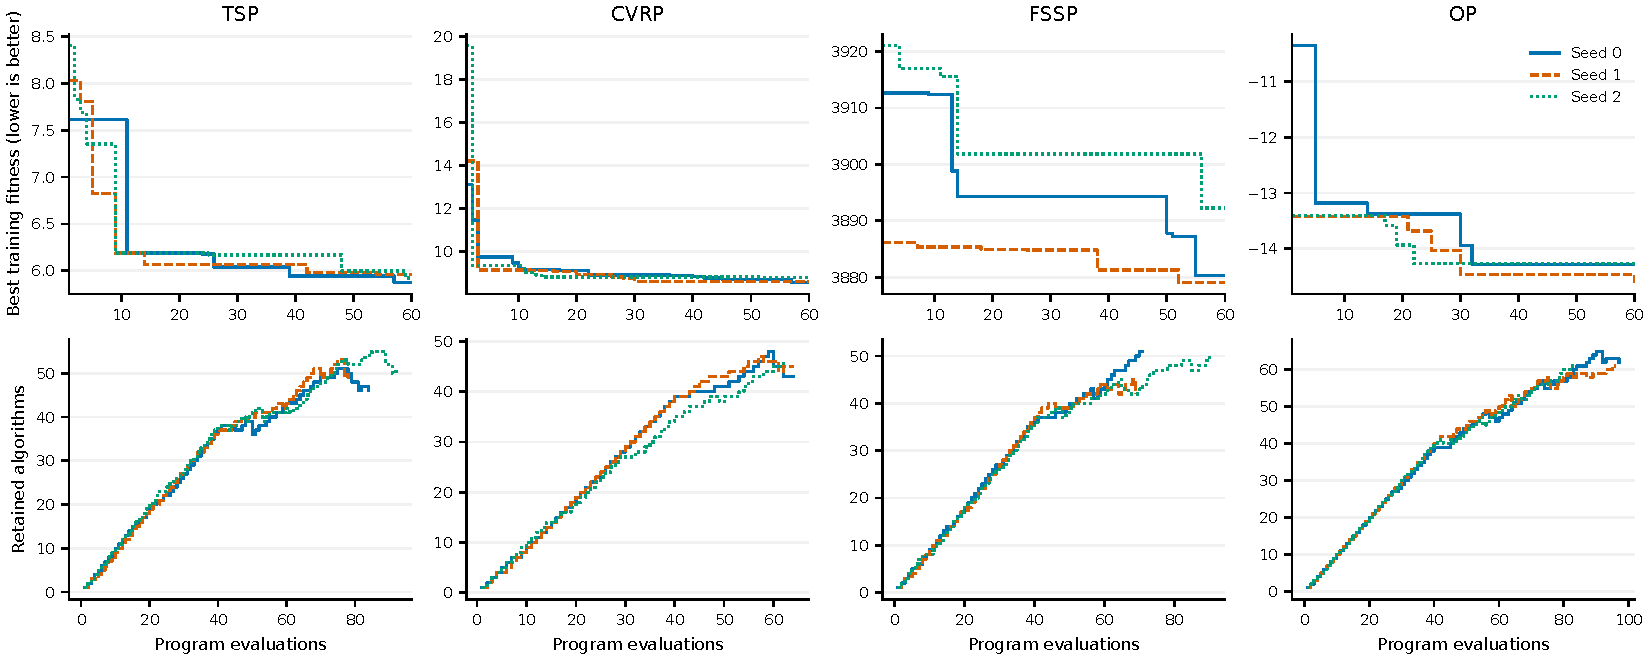
\includegraphics[keepaspectratio,alt={Early search under the frozen deployment. The upper panels show best training fitness over the first 60 evaluations, using the common observed horizon for all three seeds. The lower panels show retained algorithms after each committed evaluated insertion and any associated removals, reconstructed through each run's observed endpoint and checked against the stored tree snapshots. Thin lines identify individual seeds. These trajectories describe search and population maintenance at this early stage.}]{figures/early-search.pdf}}
\caption{Early search under the frozen deployment. The upper panels show
best training fitness over the first 60 evaluations, using the common
observed horizon for all three seeds. The lower panels show retained
algorithms after each committed evaluated insertion and any associated
removals, reconstructed through each run's observed endpoint and checked
against the stored tree snapshots. Thin lines identify individual seeds.
These trajectories describe search and population maintenance at this
early stage.}
\end{figure}

\subsubsection{4.3. How the Population Compresses
History}\label{how-the-population-compresses-history}

The frozen prefixes contain 951 evaluations and 894 committed generation
attempts. Across them, 207 updates simplify the tree. These updates
assign 286 removed implementations to 47 path regions and 175 side
regions. An audit of the recorded plans confirms that each removed node
appears in exactly one region in its update. At the observed endpoints,
the populations contain 42--62 algorithms; across runs, 608 of the 894
attached nodes remain explicit. The 40-evaluation recency window is
substantial relative to these 62--97-evaluation prefixes. Most recorded
regions are side regions (175 of 222), so the early simplification is
predominantly branch-based.

The 222 regions produce 222 model reflections, with no fallback
summaries in this snapshot. Of these regions, 186 contain one newly
removed implementation; the largest contains five. Thus, compression
commonly proceeds incrementally: a region can combine a single new
removal with experience already accumulated at its carrier. The number
of newly removed nodes measures the current update, rather than the
total history represented by the resulting summary.

Reflection calls report 505,171 input tokens and 29,283 output tokens in
total. These are model-call costs: inputs include task instructions,
endpoint code, comparisons, and inherited experience. Their ratio is not
a measure of semantic preservation. These records establish the
structural handoff from explicit implementations to node and edge
experience. The planned fixed-state comparison in Appendix E tests the
utility of that experience by holding the tree snapshot, parent,
operator, and reference fixed and changing the representation of the
same removed regions.

\subsection{5. Discussion}\label{discussion}

\textbf{The population as a representation of experience.} EvoTrace
maintains two forms of search history together. Retained programs remain
available for execution and development. Removed regions continue
through summaries whose locations preserve their developmental
relationships. A later update can change the representation again,
carrying earlier experience into a new node or edge summary. This gives
candidate maintenance a second role: organizing what subsequent
generation can learn from the search.

\textbf{Incremental compression and fidelity.} The observed region sizes
show that reflective compression often accumulates through repeated
small updates. This makes summary fidelity important across successive
handoffs. The prompts preserve explicit comparison outcomes,
actual-parent relationships, and the distinction between observations
and possible explanations. The archive provides the code and evaluations
needed to audit those accounts. An explanation of a combined
modification still concerns that tested combination; attributing its
outcome to one component requires a separate comparison.

\textbf{Scope.} The current evidence covers early search on four tasks
with one model family. It establishes the operation of structural
simplification and experience handoff. Final held-out comparisons and
controlled history-reading experiments will determine the effects on
algorithm quality and the contribution of compression.

\subsection{6. Conclusion}\label{conclusion}

EvoTrace connects candidate competition with the accumulation of design
experience. Its starting point is the distinction between an
implementation's value for further development and the value of its
history for subsequent design. A tree-structured population makes that
distinction operational: one retention decision determines the explicit
candidates, the regions to compress, and the locations that inherit the
resulting experience. Dynamic reflective simplification carries these
summaries forward as the population changes, and operator-specific views
make them available to later generation. The resulting search state
combines executable algorithms with a condensed account of their
development.

\subsection{Appendix A. Default
Settings}\label{appendix-a.-default-settings}

{\def\LTcaptype{none} % do not increment counter
\begin{longtable}[]{@{}
  >{\raggedright\arraybackslash}p{(\linewidth - 2\tabcolsep) * \real{0.5000}}
  >{\raggedright\arraybackslash}p{(\linewidth - 2\tabcolsep) * \real{0.5000}}@{}}
\toprule\noalign{}
\begin{minipage}[b]{\linewidth}\raggedright
Component
\end{minipage} & \begin{minipage}[b]{\linewidth}\raggedright
Setting
\end{minipage} \\
\midrule\noalign{}
\endhead
\bottomrule\noalign{}
\endlastfoot
Initialization; evaluation budget & Five feasible initial programs;
1,000 actual program evaluations \\
Recent retention & Fewer than 40 evaluations since birth or local
development of the node or its same-route tree parent \\
Quality representatives & Rank quality at least 0.50; best-first test
that excludes candidates superseded within their route or covered by a
representative \\
Coverage distance & Below 0.08; below 0.20 when fitness differs by at
most \(10^{-9}\) \\
Parent sampling & Sigmoid coefficient 10; local-development discount;
route maximum and within-route normalization \\
Operator prior & Refine 0.45; Crossover 0.25; Explore 0.30 \\
Reference eligibility & Rank quality at least 0.30 after excluding the
parent and identical normalized source \\
Route-view filtering & Distinct normalized entry source and AST distance
at least 0.12; latest retained version order \\
Evolution-prompt input & 30,000 tokens; whole-entry reduction when
needed \\
Generation & Temperature 1.0; maximum output 16,384 tokens \\
Reflection & Temperature 0.3; maximum output 1,536 tokens; a paragraph
of about 120 words, shorter for sparse evidence \\
\end{longtable}
}

The count \(c(v)\) includes evaluated Refine/Crossover attempts with
\(v\) as primary parent, including failed and subsequently removed
attempts. Repairs within the same attempt, Explore, read-only reference
use, reconnection, and inherited historical uses do not increment it.

The scale \(s\) in Equation (4) is the median absolute deviation with a
floor of \(10^{-6}\). If the deviation is at most \(10^{-9}\), EvoTrace
uses the median of absolute deviations larger than \(10^{-9}\), with the
same floor. If no nonzero deviation exists, the scale is the floor. The
implementation normalizes log weights at both levels; final
probabilities that underflow are represented by the smallest positive
float. A reference pool with one candidate assigns it rank quality one.

Input tokens are counted by the serving tokenizer when supplied. A
standalone client without a tokenizer uses UTF-8 byte length as a
conservative proxy and records this choice. Context fitting applies to
the three evolutionary generation prompts. Required material that still
exceeds the budget produces an explicit error.

Reflection-call or parsing failures use a deterministic summary with a
960-character budget. This fallback preserves the structural update.
Full region inputs and model responses remain archived. The search stops
early after ten consecutive attempts without a program evaluation.
Population updates are committed with their generating attempts;
restoration reads committed updates without repeating their reflection
calls.

\subsection{Appendix B. Structural Properties of One
Update}\label{appendix-b.-structural-properties-of-one-update}

Let \(K\) contain the virtual root, the actively retained nodes, and
their pairwise lowest common ancestors in a finite rooted tree.
Reconnect each retained non-root node to its nearest ancestor in \(K\).

\textbf{Connectivity and acyclicity.} Every retained node has a unique
nearest retained ancestor because its ancestor chain is totally ordered
and contains the virtual root. Every reconnected edge follows this chain
strictly upward. Repeatedly following such edges therefore reaches the
root and cannot form a cycle. The result is a rooted tree on \(K\).

\textbf{Disjoint contracted paths.} Suppose a removed node lay strictly
inside two distinct connections between retained endpoints. If the
corresponding descendant endpoints diverge below it, their lowest common
ancestor lies on the overlap and must belong to \(K\), contradicting an
unbroken removed interior. If one descendant endpoint is an ancestor of
the other, that retained endpoint interrupts the other connection. Hence
each removed intermediate belongs to one contracted path.

\textbf{Unique region assignment.} Remove these path interiors from the
set of removed nodes. Each remaining node has a unique first ancestor
outside this remaining set. That ancestor is either a path interior or a
retained node, including the root. In the first case, the node joins the
unique path region; in the second, it joins the ancestor's side region.
Every removed node is covered exactly once within the update. The
argument concerns ownership of removed implementations. Retained
endpoint code may appear as comparison context in multiple reflection
inputs.

\textbf{Best-candidate retention.} The representative selection begins
with the best feasible current node and never removes it from that set.
It therefore belongs to \(K\). This property applies to the current
population; the attempt archive independently stores the best feasible
program used for final selection.

These properties concern structure and assignment. The content of the
language summaries is determined by the reflection model and the
evidence provided to it.

\subsection{Appendix C. Reflection
Prompts}\label{appendix-c.-reflection-prompts}

Both prompts begin with a task header (problem, interface, score
direction). The evidence section lists implementations, step
differences, program-computed comparison labels, errors, and earlier
experience. The task and output sections are reproduced from
\texttt{evotrace\_v2/reflection.py}.

\textbf{Path reflection.}

\begin{quote}
Summarize the development from retained start to retained endpoint. The
program has computed each comparison label. Use these labels; do not
reconstruct scores or numerical differences. Retention does not imply
improvement. Earlier prose summaries may be wrong; current measured
comparisons take precedence.

Return one JSON object with an ``experience'' string containing a short
factual account: 1. Start with the net start-to-end outcome and name the
computational changes together. Do not substitute a last-step gain for
the net outcome. 2. Include an intermediate or side comparison only when
informative. Name both compared computations and preserve that
comparison's measured outcome label. Never say ``improved'' without
specifying which starting implementation it improved upon. 3. If the
code suggests an explanation, begin it with ``One possible explanation
for this comparison is''. Keep it specific to the implementations
tested. Combined changes do not isolate individual contributions. If the
cause cannot be distinguished, say so; no explanation is required.
Explore is an initial implementation of a new computational approach,
not local tuning of its parent. Its result concerns this draft, not the
potential of its entire approach. An unchanged score does not prove two
programs equivalent or numerically safe. Successful evaluation does not
show that faster code bought extra solver iterations. Do not conclude
with general advice, requirements, or future design instructions.
Normally use no more than 120 words; sparse evidence warrants fewer.
\end{quote}

\textbf{Side reflection.}

\begin{quote}
Summarize the experiments associated with {[}receiver{]}. Compare each
trial only to its actual parent in the evidence, never to an independent
champion or a different trial's parent. The program has computed each
comparison label; do not reconstruct scores or numerical differences.
Initial implementations without an algorithm parent have a measured
score but no parent-relative improvement. Earlier prose summaries may be
wrong; current measured comparisons take precedence.

Return one JSON object with an ``experience'' string containing a short
factual account: 1. Name the starting computation, the tested changes
together, and the observed outcome using the measured comparison label.
Explore is an initial implementation of a new computational approach,
not local tuning of its parent. Its result concerns this draft, not the
potential of its entire approach. 2. If the code suggests an
explanation, begin it with ``One possible explanation for this
comparison is''. Keep it specific to the implementations tested.
Combined changes do not isolate individual contributions. If the cause
cannot be distinguished, say so; no explanation is required. Preserve
useful earlier observations only when their comparison and conditions
are clear. An unchanged score does not prove two programs equivalent or
numerically safe. Successful evaluation does not show that faster code
bought extra solver iterations. Do not conclude with general advice,
requirements, or future design instructions. Normally use no more than
120 words; sparse evidence warrants fewer.
\end{quote}

\subsection{Appendix D. Reproducibility and
Accounting}\label{appendix-d.-reproducibility-and-accounting}

The current deployment freezes the method source, task definitions,
evaluator, and sampling configuration before launch. Every committed
attempt records its generated program, all evaluations including repair,
the parent and reference identifiers, the context view, and the
population update. Recorded updates include the removed regions,
reflection responses, and the resulting tree. Recovery replays committed
updates without repeating their model calls. The final evaluated version
of an attempt enters the online tree; earlier repair versions remain in
the attempt archive.

The experiment uses seeds 0, 1, and 2 for search. TSP training uses
50-node Euclidean instances with data seed 2024. CVRP uses 30 ants and
100 ACO iterations; OP uses 20 ants and 50 iterations. Both ACO tasks
use solver seed 1234. The training evaluator seed is 730241. The
complete frozen task configuration determines FSSP instances and solver
settings. Search prompts expose the interface and objective; instance
counts, dataset splits, and solver iteration settings remain evaluation
conditions rather than generation instructions.

Generation sampling additionally sets top-p to 0.8, top-k to 20, and
presence penalty to 1.5. The shared serving pool routes calls among
endpoints; returned model identifiers include both \texttt{Qwen3.8-27B}
and \texttt{qwen3.8-27b-awq}. Endpoint identifiers alone do not
establish identical numerical inference. Request metadata records the
selected endpoint and returned usage for each call. Provider errors are
accounted for separately from candidate execution failures.

The supplied evidence snapshot stores per-run source paths, SHA-256
hashes of the committed attempt files, capture time, configurations
without credentials, and the exact evaluation prefixes used in Section
4. The score table and Figure 3 are generated from this snapshot.
Updating the snapshot is an explicit operation; rebuilding the paper
does not refresh experimental data.

\subsection{Appendix E. Evaluation Design for the Core
Claim}\label{appendix-e.-evaluation-design-for-the-core-claim}

The following protocol specifies the remaining tests. The results in
Section 4 comprise the observed deployment snapshot.

\textbf{Complete search.} Freeze all compared methods before running
three search seeds per task. Align task interfaces, datasets,
candidate-evaluation limits, generation settings, evaluation accounting,
and final selection. Record native budget conventions for methods whose
published procedure counts generations rather than evaluations. Report
best training trajectories, test scores of the training-selected
program, all seed-level values, failures, and generation, repair, and
reflection costs.

\textbf{Fixed-state history representation.} Sample states from declared
evaluation checkpoints without selecting for later success. Hold the
parent, operator, reference, current code, and task instructions fixed.
Compare omitted history, raw material from the same removed regions, and
the actual reflected summaries. Use repeated samples per condition and
treat the snapshot as the pairing unit; descendants sampled from one
snapshot are not independent search runs. Report fitness, execution
success, improvement over the parent, and measured input tokens by task
and operator. Report raw histories that exceed the input window
separately.

\textbf{Experience placement.} Keep the selected summaries and the input
budget fixed, then compare their original structural presentation with a
shared list that preserves source labels. This comparison separates the
effect of explicit structural grouping from the mere availability of
text.

\textbf{Summary fidelity.} Select reflections by a recorded random
sample across task, region type, and number of earlier handoffs. Check
comparison direction against the evaluation archive and computational
descriptions against code. Distinguish errors in measured outcomes, code
descriptions, and proposed explanations. Trace later prompt exposure
separately from any claim that the experience caused an improvement.

\bibliography{references.bib}

\end{document}
